\section{Správa paměti, statické přidělování paměti, dynamické přidělování paměti, garbage collector, reprezentace informace v~paměti.}

Každá paměť, která je přiřazena procesu se~dělí na~4 základní bloky:

\begin{multicols}{2}
	\begin{itemize}[noitemsep]
		\item Segment instrukcí(Code)/Kódová oblast
		\item Datový segment(Data)/Datová oblast
		\item Halda/hromada(Heap)
		\item Zásobník(Stack)
		\vfill
	\end{itemize}
	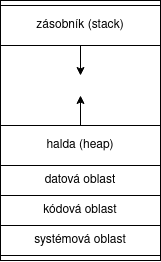
\includegraphics[scale=0.3]{images/pamet.png}
\end{multicols}

\textbf{Code} je množina strojových instrukcí, které naprosto jednoznačně provádí program. Dle těchto instrukcí PC postupuje ve~výpočtu.

V~části \textbf{Data} můžou být uložena data, která jsou známa při~překladu programu (hodnoty polí, konstant, proměnných, některé textové řetězce).

Bloky Code a~Data jsou známy v~době překladu a~jejich velikost se~v~průběhu nemění.

\textbf{Heap} slouží k~alokaci dynamické paměti. Je založena na~stromové datové struktuře. Obsahuje objekty a~instance proměnných (atributy třídy).

\textbf{Stack} je důležitý pro~volaní správných funkcí. Funguje na~principu LIFO. S~uložením funkce na~stack se~posunuje ukazatel na~pozici v~registru (\emph{stack pointer}). Po~dokončení té funkce je odstraněna ze~zásobníku a~ukazatel změněn na~předchozí funkci. Obsahuje metody/funkce, lokální proměnné a~reference na~proměnné%
\footnote{Video k~vysvětlení stacku: \url{https://www.youtube.com/watch?v=uwV0hotRrLw}}.

Bloky Heap a~Stack jsou dynamické a~jejich velikost roste/zmenšuje se~u~každého jiným směrem v~průběhu programu.

\subsection{Statické přidělování paměti}

Staticky se~ukládají datové struktury, které jsou definovány při~překladu programu. K~jednotlivým paměťovým úsekům lze přistupovat pomocí názvu proměnné. V~průběhu se~adresa nemůže měnit.

\subsection{Dynamické přidělování paměti}

Dynamicky se~paměť přiděluje na~základě požadavku při~průběhu programu. K~dynamicky přidělenému paměťovému úseku se~dá přistoupit pouze nepřímo pomocí ukazatele. Ukazatel je součástí statické nebo dynamické struktury. Dynamicky přidělovaná paměť se~čerpá z~vyhrazeného prostoru paměti počítače.

\subsubsection{Dynamické přidělování paměti bez~regenerace}

Regenerace paměti je její pročištění od~nepoužívaných částí paměti.

Dynamické přidělovaní paměti bez~regenerace přiděluje požadované úseky postupně tak jak Jsou za~sebou umístěny až do~vyčerpaní vyhrazené paměti. Využívá pracovního ukazatele, který ukazuje na~první adresu volné paměti. Nejčastěji pomocí operace "new" zapíše do~paměti a~změní ukazatel na~novou hodnotu, která ukazuje na~novou adresu volné části a~v indikátoru paměti hodnotu obsazení označí \emph{true}. Operace \enquote{free/delete} okamžitě neuvolní paměť, ale přepíše indikátor paměti na~\emph{false}; regenerace probíhá později po~větších částech.

\subsubsection{Dynamické přidělování paměti s~regenerací}

Na~rozdíl od~dynamického přidělovaní bez~regenerací se~zde regeneruje pro~každé operaci \enquote{free/delete}. S~tím přichází problém s~fragmentací paměti. Po~uvolnění paměti by tyto části mohly vytvářet sekvence malých, oddělených a~přitom sousedních prvků. Často je defragmentace těchto volných bloků spojena s~operací \enquote{free/delete}. Snaží se~slučovat volné úseky se~sousedními volnými úseky.

\subsection{Garbage collector}

Je nejpokročilejším způsobem dynamického přidělovaní paměti. Oproti předchozím způsobům je méně efektivní. Skládá se~ze~tří fází:

\begin{itemize}[noitemsep]
	\item \textbf{Allocation} přiděluje po~sobě jdoucí úseky stejně jako metoda bez~regenerace až do~vyčerpání celého vyhrazeného prostoru.
	\item \textbf{Marking} nastává pouze pokud je vyčerpán celý prostor. Prochází prostorem a~vyhledává a~označuje úseky, které nejsou aktivní a~jejich návrat do~společné paměti způsobí regeneraci.
	\item \textbf{Garbage collecting}: provádí se defragmentace přesunem všech uvolněných úseků do~jednoho souvislého úseku. Tím se~vytvoří nový souvislý úsek pro~alokaci.
\end{itemize}

Tyto tři fáze se~opakují dokola, dokud nedojde k~situaci, že nový úsek není dostačující pro~fázi alokace. Z~tohoto důvodu dojde k~ukončení programu.

\paragraph{Reprezentace informace v~paměti} Pokud je datový typ primitivní, je uložen na~přímo v~paměti a~u objektů je reprezentován pouze ukazatelem na~místo v~paměti%
\footnote{Zatímco jeden \textit{integer} v~paměti zabere 32bitů, \textit{objekt} (v~C si lze představit jako \textit{struct}) obsahující dva integery bude v~paměti reprezentován jako \textit{odkaz} (pointer) na~část paměti kde začíná první integer. Nedá se~úplně s~jistotou říct, že zabere 64bitů, jelikož se~zpravidla dodá padding pro~metadata).}%
.

\clearpage
\section{Jazyk UML a~objektově orientovaný návrh - dědičnost, generalizace, asociace 1:n, n:1, n:n, agregace a~kompozice.}

\textbf{Jazyk UML} je grafický jazyk pro~popis programových systémů. Slouží pro~vizualizaci, specifikaci, návrh a~dokumentaci systémů. K~zobrazení se~využívají diagramy, kde nejčastěji používané jsou:

\begin{enumerate}[noitemsep]
	\item Strukturální
	\begin{enumerate}[noitemsep]
		 \item Diagram tříd
		 \item Diagram případů užití
		 \item Diagram komponent
		 \item Diagram nasazení
	\end{enumerate}
	\item Behaviorální
	\begin{enumerate}[noitemsep]
		 \item Diagram aktivit
		 \item Diagram sekvencí
		 \item Diagram stavů
	\end{enumerate}
\end{enumerate}

Nejpoužívanější jsou diagramy tříd a~případů užití. Diagram tříd popisuje strukturu systému, znázorňuje datové struktury a~operace u~objektů a~souvislosti mezi nimi. Skládá se~z~tříd, rozhraní, abstraktních tříd. Tyto tři prvky se~dále skládají z~názvu třídy/rozhraní, atributů (rozhraní neobsahuje atributy), a~operace (metody/funkce) Diagram případů užití se~nejčastěji používá při~komunikaci se~zákazníkem a~méně technicky znalou stranou. Skládá se~z~herců (\emph{actor}) a~případů užití a~systém. Tyto strany jsou propojeny jak mezi sebou, tak i~sami se~sebou pomocí těchto propojení\,--\,asociace, generalizace, rozšíření vztahu, vztah zahrnuje.

\textbf{Objektově orientovaný návrh} je jeden ze~způsobů jak reprezentovat informaci. Vychází z~principů reálného světa, neboli je jednoduše srozumitelný pro~člověka. Není spojen s~žádným programovacím jazykem, ale jazyk, který bude použit pro~implementaci, musí splňovat objektově orientované principy. Výhodou OON může být, že při~návrhu lze určit co jaká část programu komunikuje z~jakou a~co každá dělá, takže se~sníží počet chyb v~kódu a~tím i~náklady. OON se~nezabývá konkrétní implementací, ale pouze vazbami mezi objekty.

OON přístup není vhodné využívat pokud na~cílové platformě neexistuje překladač OOP jazyka, návrh je určen pro~jazyk nepodporující OOP nebo by přepis stávajícího kódu byl neekonomický, hlavně u~projektů s~krátkou životností.

\subsection{Vztahy mezi třídami}

\textbf{Závislost} je dynamický a~zároveň nejslabší vztah. Ukazuje jak co na~sobě závisí. \\
\includegraphics[scale=1]{images/zavislost.PNG}

\textbf{Asociace} je pevný vztah. Určuje vztah mezi dvěma prvky, které mohou existovat nezávisle na~sobě. Asociace může mít směr od~jednoho prvku k~druhému nebo obousměrně. Objekt ve~směru šipky může nalézt odkaz na~následujíc objekty. \\
\includegraphics[scale=1]{images/asociace.PNG}

\textbf{Násobnost asociací} určuje kolik vazeb může mít danný objekt. Například $1:n$ může být 1 objekt a~ten mít reference na~$n$ objektů ke~kterým má asociaci (faktura$:n \cdot$ položka).

\textbf{Agregace} je typ asociace. Reprezentuje vztah typu celek--část. Zde je u~celku umístěn kosočtverec. Celek je entita, která drží kolekci prvků. Část může existovat bez~celku nebo být součástí jiných kolekcí. \\
\includegraphics[scale=1]{images/agregace.PNG}

\textbf{Kompozice} je typ asociace. Je to nejsilnější vztah a~je podobná agregaci, s~rozdílem v~tom, že část nemá bez~celku smysl. Pokud zanikne celek, zaniknou i~části. U~celku je násobnost vždy 1. \\
\includegraphics[scale=1]{images/kompozice.PNG}

\textbf{Dědičnost/generalizace} se využívá jestliže mají některé třídy společné vlastnosti. Tím například nemusíme vytvářet duplicitní kód. Směr šipky udává od~koho třída dědí (obrázek B dědí z~A). Díky tomuto lze jednodušeji rozšířit třídu o~atributy a~operace. Neplést si z~asociací, se~kterou jinak nesouvisí. \\
\includegraphics[scale=1]{images/dedicnost.PNG}

\clearpage
\section{Třídy složitosti paměťové a~časové. Notace Theta. Notace Omega. Notace velké-O. Asymptotický popis složitosti algoritmu. Posouzení složitosti algoritmů.}

\subsection{Teorie vyčíslitelnosti}

Zkoumá otázku algoritmické řešitelnosti problému, ne z~pohledu času ale jestli jdou vůbec řešit. Vyčíslitelnost je zkoumána pomocí teoretických výpočetních modelů\,--\,deterministický a~nedeterministický konečný automat, zásobníkový automat, Turingův stroj a~další.

Složitost je vztah algoritmu k~prostředkům (čas a~velikost paměti). Paměťová složitost je závislost paměťových nároků na~vstupních datech, zatímco časová je dána hrubým odhadem počtu kroků, který daný algoritmus musí provést na~základě délky vstupních dat. Měli by se~brát v~potaz oba dva typy složitosti, jelikož může nastat že máme dva algoritmy na~řešení daného problému a~jeden má menší časovou složitost a~druhý zase paměťovou. Zde výběr z~těchto složitostí závisí hlavně na~tom kde bude daný algoritmus implementován.

\subsection{Asymptotická složitost}

Jelikož vždy nelze určit přesnou složitost algoritmu, byla vyvinuta asymptotická složitost. Tato složitost aproximuje chovaní funkce ze~tří pohledu:

\begin{itemize}[noitemsep]
	\item Nejlepší případ $\Omega$ (Omega) značí spodní hranici trvání algoritmu.
	\item Průměrný případ $\Theta$ (Theta) odhaduje nejpravděpodobnější dobu trvání algoritmu.
	\item Nejhorší případ notace O (Omicron, big-O) značí horní hranici trvání algoritmu. Je nejčastěji používaná.
\end{itemize}

\begin{table}[h]
	\begin{tabularx}{\textwidth}{|c|c|X|}\hline
		Konstantní & O(1) & Nezávisí na~velikosti vstupních dat \\\hline
		Logaritmická & O($\log{n}$) & Počet operací odpovídá logaritmu např. vstup 1\,000\,000\,000 $==$ 30 operací \\\hline
		Lineární & O($n$)& počet operací je závislý na~velikosti vstupních dat \\\hline
		Kvazilineární& O($n\log{n}$)& Zástupce quicksort \\\hline
		Kvadratická& O($n^2$)& Např 500 vstupů $==$ 250\,000 operací \\\hline
		Kubická & O($n^3$)& Např. 200 vstupů $==$ 8\,000\,000 operací \\\hline
		Exponenciální&O($2^n$)& Exponenciální růst počtu operací \\\hline
		Faktoriální&O($n!$)& Faktoriální růst počtu operací \\\hline
	\end{tabularx}
\end{table}

\textbf{Polynomiální algoritmy} jsou takové algoritmy jejichž notace v~big-O je ohraničena polynomiální funkcí shora. Spadají zde například $\log{n}$, $k*n$, $3n^3 + 4n$, $2*n\log{n}$ a~podobné. Nepatří sem exponenciální, faktoriální a~jim podobné. Abychom algoritmus označili jako efektivní, jeho vykonání by mělo být možné v~polynomiálním čase, jinak ho lze označit jako neefektivní. Při~vysokých hodnotách v~kryptografii by nepolynomiální algoritmy byly nepoužitelné.

\subsection{Posouzení složitosti algoritmů}

Vybrané algoritmy a~jejich složitost jsou popsány v~dalších otázkách. Zde jsou jenom lehce shrnuty; složitost je udávána z~pohledu časové složitosti.

\subsubsection{Algoritmy řazení}

Třídění pomocí algoritmů Bubble Sort, Insert Sort a~Select Sort má složitost O($n^2$). Algoritmus Quick Sort má složitost $\theta$($n\log{n}$), kdy v~nejhorším případě může nabývat až O($n^2$). Algoritmus Merge Sort má složitost O($n\log{n}$).

\subsubsection{Algoritmy hledaní}

Binární vyhledávání má složitost O($\log{n}$) a~lineární/sekvenční má složitost O($n$).

\subsection{Třídy složitosti}

Vyjadřuje jak náročný je výpočet je nezbytný k~vyřešení problému. \\
Rozdělení:
\begin{itemize}[noitemsep]
	\item Třída P\,--\,schůdné algoritmy. Jsou proveditelné v~polynomiálním čase na~deterministickém turingově stroji.
	\item Třída NP\,--\,neschůdné algoritmy. Je možné je provést v~polynomiálním čase na~\textbf{nedeterministickém} TS (nebyl doposud sestaven). Spadají pod ně i~všechny algoritmy z~třídy P
	\item Třída NP-těžké\,--\,přinejmenším tak těžké, jako nejtěžší z~NP. Nemusí být vykonatelné pomocí TS.
\end{itemize}

\subsection{Turingův stroj}

\begin{itemize}[noitemsep]
	\item Turingův stroj\,--\,nelze měnit program.
	\item Univerzální Turingův stroj\,--\,lze přepsat program, dnešní pc, mobil atd.
	\item Nedeterministický Turingův stroj\,--\,doposud nesestaven, sestrojení by znamenalo konec asymetrické kryptografie, neví se~jestli ho lze vůbec sestrojit (P vs PN).
	\item Paralelní Turingův stroj\,-\,z pohledu vyčíslitelnosti je ekvivalentní s~běžným jen přináší více výkonu.
	\item Kavantový Turingův stroj\,--\,založen na~superpozicích stavů, dokáže řešit \uv{exponenciální explozi} a~převést ji na~problém se~složitostí v~polynomiálním čase.
\end{itemize}

\clearpage
\section{Posouzení složitosti algoritmu vyhledávání. Srovnání lineárních a~nelineárních struktur. Vztah časové a~paměťové složitosti. Abstraktní datový typ (ADT). ADT lineární seznam. ADT cyklický seznam. Operace vkládání, mazání a~vyhledávání prvku v~ADT lineární seznam. ADT zásobník, ADT fronta.}

\subsection{Algoritmy hledání}

Dva základní algoritmy pro~hledání jsou \textit{Binary search}%
\footnote{Binární vyhledávání funguje na~principu půlení seřazeného seznamu. Pokud je hledaná hodnota menší než střední hodnota, vyhledává se v~první polovině, pokud je větší tak v~druhé. Takto se iteruje dokud není číslo nalezeno. Více např. \url{https://en.wikipedia.org/wiki/Binary_search_algorithm}.} %
a~\textit{Linear search}%
\footnote{Lineární vyhledávání je naprosto jednoduchý lineární průchod seznamem, kde se~postupně hledá požadovaná hodnota. Alternativa je \emph{Linear Sentinel search}, která přidá hledanou hodnotu na~konec seznamu. Více např. \url{https://www.geeksforgeeks.org/linear-search/} nebo \url{https://algorithmoftheweek.blog/2020/06/10/sentinel-linear-search/}.}%
. \textit{Binary} funguje lépe než \textit{Linear} ale pouze pro~větší seznamy, zároveň je třeba předem seznam seřadit.

\begin{table}[h]
	\centering
	\caption{Big-O složitosti vyhledávacích algoritmů}
	\begin{tabular}{|c|c|c|}\hline
		Algoritmus & Časová & Paměťová\\\hline
		Linear Search & O($n$) & O($1$)\\\hline
		Binary Search & O($\log n$) & O($1$)\\\hline
	\end{tabular}
\end{table}

\subsection{Lineární a~nelineární struktury}

\textbf{Lineární} jsou pole, seznamy, zásobník, fronta.

\begin{table}[h]
	\centering
	\caption{Složitost akcí v~lineárních strukturách}
	\begin{tabular}{|c|c|c|c|c|}\hline
		Struktura & Přidat & Vyhledat & Smazat & Výběr dle indexu\\\hline
		Pole & O($n$) & O($n$) & O($n$) & O($1$) \\\hline
		Seznam & O($1$) & O($n$) & O($n$) & O($n$)\\\hline
		Pole proměnlivé délky & O($1$) & O($n$) & O($n$) & O($1$) \\\hline
		Zásobník & O($1$) & -- & O($1$) & -- \\\hline
		Fronta & O($1$) & -- & O($1$) & -- \\\hline
	\end{tabular}
\end{table}

\textbf{Nelineární} jsou například stromy, které, pokud jsou nějak vyvažovány, mají náročnost O($\log{n}$). Pokud se~nevyvažují, náročnost je O($n$). Tyto složitosti jsou pro~všechny operace stejné.

\subsection{Vztah časové a~paměťové složitosti}

Většina algoritmů je kompromisem mezi těmito dvěma druhy složitosti. Pokud bychom měli algoritmus s~vysokými nároky na~časovou složitost (aby byl co nejrychlejší) tak jeho paměťová složitost bude vzrůstat. Většinu algoritmů je nějakým způsobem optimalizovaná nebo ji lze optimalizovat.

\subsection{Abstraktní datový typ}

Abstraktní datový typ je množina druhů dat (hodnot) a~příslušných operací, které jsou přesně specifikovány a~to nezávisle na~konkrétní implementaci. ADT je reprezentováno rozhraním, kde uživatele tohoto rozhraní zajímá pouze, jak se~používá a~ne jak je implementováno. Poté, co je konkrétní ADT implementován v~programovacím jazyce, stává se~z~něj datová struktura.

ADT dělíme podle počtu datových položek na~statický a~dynamický datový typ. Statický datový typ má neměnnou velikost a~dynamický mění velikost dle provedené operace. Dále se~dělí dle jednoznačného bezprostředního následníka na~lineární a~nelineární. Lineární mají následníka a~u nelineárních neexistuje přímý jednoznačný následník.

\textbf{Dělení ADT:}
\begin{itemize}[noitemsep]
	\item Lineární
	\begin{itemize}[noitemsep]
		 \item Pole\,--\,statický
		 \item Seznam\,--\,dynamický
		 \item Zásobník\,--\,dynamický
		 \item Fronta\,--\,dynamický
	\end{itemize}
	\item Nelineární
	\begin{itemize}[noitemsep]
		 \item Strom\,--\,dynamický
		 \item Množina (Set)\,--\,dynamický
	\end{itemize}
\end{itemize}

\subsection{Lineární seznam}

ADT lineární seznam je seznam, kde každý uzel má unikátního následníka. Výhodou lineárního seznamu efektivní vkládání a~mazání, neefektivní je přístup k~prvkům. Na~rozdíl od~pole, jehož vlastností je rychlá indexace prvků. Každý prvek lineárního seznamu obsahuje data a~ukazatel na~další prvek v~seznamu.

\begin{figure}[ht]
	\centering
	\includegraphics[scale=0.5]{images/linsez.PNG}
\end{figure}

Možné operace s~ADT seznamem:
\begin{itemize}[noitemsep]
	\item Nalezení délky N seznamu
	\item Výpis všech prvků seznamu
	\item Vytvoření prázdného seznamu
	\item Získaní k-tého prvku ze~seznamu
	\item Vložení novéhé prvku za~k-tý prvek seznamu
	\item Smazaní prvku ze~seznamu
	\item Nalezení následujícího prvku za~aktuálním v~seznamu
	\item Nalezení předchozího prvku před aktuálním v~seznamu
\end{itemize}

\paragraph{Cyklický lineární seznam} Je stejný jako lineární ale poslední prvek nemá ukazatel null ale odkaz na~první prvek seznamu.

\begin{figure}[ht]
	\centering
	\includegraphics[scale=0.5]{images/cycsez.PNG}
\end{figure}

\paragraph{Obousměrně vázaný lineární seznam} Nemá pouze ukazatel na~další prvek ale i~na~předchozí. Umožňuje procházení v~obou směrech.

\begin{figure}[ht]
	\centering
	\includegraphics[scale=0.5]{images/obousez.PNG}
\end{figure}

\paragraph{Vkládaní do~lineárního seznamu} Vložení prvku na~určitou pozici funguje tak, že se~najde pozice k~kde se~zde vloží prvek který bude odkazovat na~prvek, který byl předtím na~pozici k~a~v prvku k-1 se~přepíše ukazatel na~nový prvek. Operace fungují stejně jen jsou vázány na~obě strany.

\begin{figure}[ht]
	\centering
	\includegraphics[scale=0.5]{images/sezins.PNG}
	\caption{Vkládání do~lineárního seznamu.}
	
	\includegraphics[scale=0.5]{images/sezinsfirst.PNG}
	\caption{Vkládání do~lineárního seznamu na~první pozici. Ukazatel pole se~přepisuje na~první prvek a~ve vkládaném prvku se~přidá ukazatel na~předchozí první prvek.}

	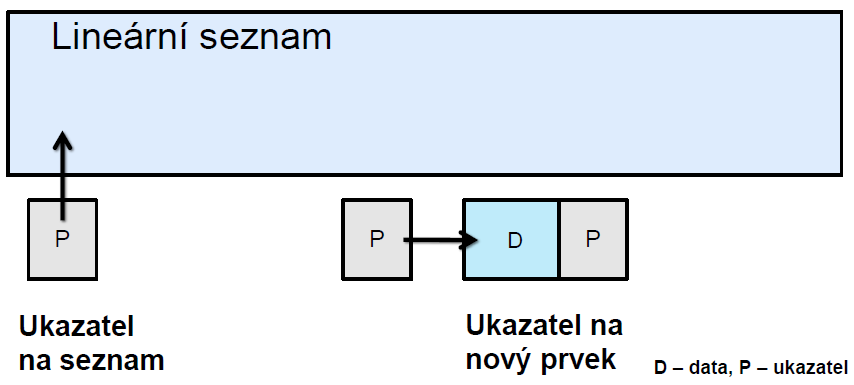
\includegraphics[scale=0.5]{images/sezinsempty.PNG}
	\caption{Vkládání do~prázdného lineárního seznamu.}
\end{figure}

\paragraph{Mazaní v~lineárním seznamu} Prvek $k-1$ přepíše ukazatel na~prvek $k+1$. U~prvního prvku se~přepíše pouze ukazatel na~další prvek.

\begin{figure}[ht]
	\centering
	\includegraphics[scale=0.5]{images/sezdel.PNG}
	\caption{Mazání v~lineárním seznamu}
\end{figure}

\paragraph{Vyhledávaní v~lineárním seznamu} Vyhledávat se dá podle prvku nebo podle dat. Pomalu iteruje seznamem dokud nenarazí na~ten prvek nebo konec seznamu. U~obousměrného se~dá hledat od~začátku a~od konce.

\subsection{Zásobník}

Dynamická datová struktura umožnující vkládaní a~odebírání hodnot tak, že naposledy vložená hodnota se~odebere jako první (LIFO). Základní operace jsou \enquote{Vložení na~vrchol}, \enquote{Odebraní z~vrcholu} a~\enquote{Test na~prázdnost zásobníku}.

\subsection{Fronta}

Dynamická datová struktura, kde se~odebírají prvky v~tom pořadí v~jakém byli vloženy (FIFO). Základní operace jsou stejné jako u~zásobníku. Existuje tzv. prioritní fronta, která funguje na~principu fronty ale bere z~ní podle priority.

\clearpage
\section{Abstraktní datový typ strom. Abstraktní datový typ binární strom. Úplný binární strom. Abstraktní datový typ binární vyhledávací strom (operace vložení, odstranění, smazání uzlu stromu). Průchody stromy in-order, pre-order, post-order.}

\textbf{ADS typu strom} je nelineární dynamická abstraktní datová struktura. Každý uzel stromu může mít $n$ potomků a~zároveň má pouze jednoho předka. Nejčastější zástupci jsou obecný strom nebo $n$-ární strom. $n$-ární má maximální počet potomků rovný $n$, obecný strom není počtem potomků omezen. Skládá se~z~uzlů, které se~pojmenovávají:

\begin{itemize}[noitemsep]
	\item Kořen, který existuje pouze jeden. Je to uzel bez~předchůdce.
	\item Listy jsou to uzly, které nemají následníka
	\item Vnitřní uzly jsou ty, které nejsou kořenem ani listem stromu.
\end{itemize}

\begin{figure}[ht]
	\centering
	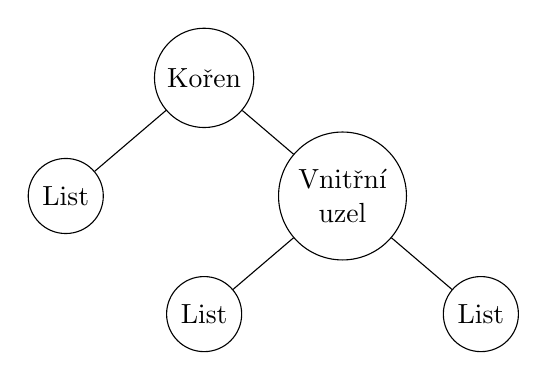
\begin{tikzpicture}[
		sibling distance=10em,
		every node/.style = {shape=circle,
		draw, align=center,
		top color=white, bottom color=white}
	]
	\node {Kořen}
		child { node {List} }
		child { node {Vnitřní\\uzel}
			child { node {List}}
			child { node {List}}};
	\end{tikzpicture}
	\caption{Binární strom}
\end{figure}

\subsection{Binarní strom}

Binární strom je strom, který má nanejvýše dva potomky na~jeden uzel. Za~\textbf{úplný binární strom} se~považuje binární strom, který se~plní po~úrovni hloubky z~levé strany. Dokud není plně zaplněn levý potomek, nezaplní se pravý%
\footnote{Ukázka úplného binárního stromu např. \url{https://home.cs.colorado.edu/~main/supplements/pdf/notes10a.pdf}.}.

\subsection{Binarní vyhledávací stromy}

U~těchto stromů musí platit, že levá část potomků musí být vždy menší než kořen a~pravá část vždy vetší, tzn. prvky jsou seřazeny. Tyto stromy mohou být nevyvážené ale častěji se~také vyvažují, aby bylo dosaženo jejich optimální složitosti O($\log{n}$). Mohl by totiž nastat případ, kdy by ze~stromu vznikl pouze strom.

\begin{figure}[ht]
	\begin{minipage}[b]{0.47\textwidth}
		\centering
		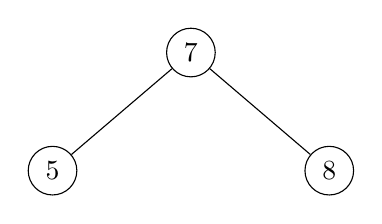
\begin{tikzpicture}[
			sibling distance=10em,
			every node/.style = {shape=circle, draw, align=center, top color=white, bottom color=white}
		]
		\node {7}
			child { node {5} }
			child { node {8}
		};
		\end{tikzpicture}
		\caption{Vyvážený strom}
		\label{even_binary_tree}
 	\end{minipage}
	\hspace*{1em}%
 	\begin{minipage}[b]{0.47\textwidth}
 		\centering
		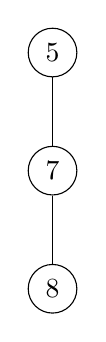
\begin{tikzpicture}[
			sibling distance=10em, every node/.style = {shape=circle, draw, align=center, top color=white, bottom color=white}
		]
		\node {5}
			child { node {7}
		  		child { node {8} } 
		  	};
		\end{tikzpicture}
		\caption{Nevyvážený strom}
		\label{noneven_binary_tree}
	\end{minipage}
\end{figure}

U~nevyvážené stromu na~obrázku \ref{noneven_binary_tree} lze vidět, že by se~jednalo spíše o~seznam. U~vyvážených binárních stromů by rozdíl hloubky levé a~pravé části měl být 0 nebo 1.

\paragraph{Vyhledávaní v~binárních vyvážených stromech} Postupuje se~od~kořene směrem dolů, kde se~porovnává jestli prvek bude v~levém nebo pravém uzlu, pokud to už není hledaný prvek. Tak se~postupuje vždy na~každém navštíveném uzlu dokud není nalezena hledaná hodnotu nebo konec uzlu. Při~hledání min/max se~algoritmus vydává doleva/doprava dokud nenarazí na~uzel, který má svůj levý/pravý uzel roven \emph{null}.

\paragraph{Vložení do~binárních stromů} Postup je stejný jako při~vyhledávání. Vkládá se pokud je nalezena hodnota \emph{null} nebo položka se~stejnou hodnotou (v~tom případě ji implementace může a~nemusí přepsat).

\paragraph{Odstranění prvků} Pokud uzel nemá žádné potomky, pouze se odstraní a~z jeho rodiče se~smaže jeho reference. Pokud má jehoho potomka, reference v~rodiči se změní na~referenci tohoto potomka. Pokud má potomky dva, existují dvě možnosti: PL a LP.

Pro~pravý prvek (PL) nalezneme uzel, který je nejvíc napravo v~levém stromu a~ten zaměníme za~uzel, který chceme smazat: nejpravější uzel v~levém stromu převezme referenci ze~mazaného uzlu a~rodič mazaného uzlu změní referenci na~nejpravější uzel levého stromu. Pro levý prvek (LP) je to podobné, jen se~vybírá nejlevější uzel z~pravého stromu. Viz obrázky \ref{treePL} a~\ref{treeLP}.

\begin{figure}[ht]
	\centering
	\includegraphics[scale=0.8]{images/treePL.PNG}
	\caption{Odstranění prvku s~využitím PL.}
	\label{treePL}

	\includegraphics[scale=0.8]{images/treeLP.PNG}
	\caption{Ostranění prvků s~využitím LP.}
	\label{treeLP}
\end{figure}

\subsection{Procházení stromů}

Strom a~výsledky procházení jsou na~obrázku \ref{tree}.

\begin{enumerate}[noitemsep]
\item \textbf{Pre-order}. Nejprve se zpracuje kořen, poté levý podstrom a~nakonec pravý podstrom. Využívá se k~vytváření kopií stromů.
\item \textbf{In-order}. Nejprve se zpracuje levý podstrom, poté kořen a~nakonec pravý podstrom. Výsledkem je seřazený seznam.
\item \textbf{Post-order}. Nejprve je zpracován levý podstrom, poté pravý a~nakonec kořen. Využívá se k~mazání stromu od~listů ke~kořenu.
\end{enumerate}

\begin{figure}[ht]
	\centering
	\includegraphics[scale=1]{images/tree.PNG}
	\caption{
		Čteční stromu. \\
		\textbf{Pre-order}: 5, 2, 4, 3, 15, 9, 7, 11, 12, 17. \\
		\textbf{In-order}: 2, 3, 4, 5, 7, 9, 11, 12, 15, 17. \\
		\textbf{Post-order}: 3, 4, 2, 7, 12, 11, 9, 17, 15, 5. \\
	}
	\label{tree}
\end{figure}

\clearpage
\section[Problematika nevyvážených stromů. Vyvažování stromů AVL - rotace: jednoduchá levá, jednoduchá pravá, dvojitá levá, dvojitá pravá. Red-Black stromy]{Problematika nevyvážených stromů. Vyvažování stro-mů AVL -- rotace: jednoduchá levá, jednoduchá pravá, dvojitá levá, dvojitá pravá. Red-Black stromy.
}

Nevyvážený strom je problematický v~tom, že jeho složitost může klesnout až na~O($n$) z~O($\log{n}$). Z~tohoto důvodu má smysl stromy vyvažovat.

Vyvážený strom má hloubku levého a~pravého podstromu rovnou vždy 0 nebo 1. Pokud má hloubku větší tak se~označuje za~nevyvážený a~z pohledu problematiky by se~měl vyvážit například metodou AVL nebo Red-Black stromy.

\subsection{AVL stromy}

Jsou dobře vyvážené ale hrozí zde problém mnohonásobné rotace, takže vkládání může být méně efektivní. Mají velice efektivní vyhledávání.

Vyvažuje se~dvěma typy rotace, u~kterých pak dále rozlišujeme stranu%
\footnote{Vizualizace \url{https://www.cs.usfca.edu/~galles/visualization/AVLtree.html}.}.

\begin{figure}[ht]
	\begin{minipage}[b]{0.47\textwidth}
		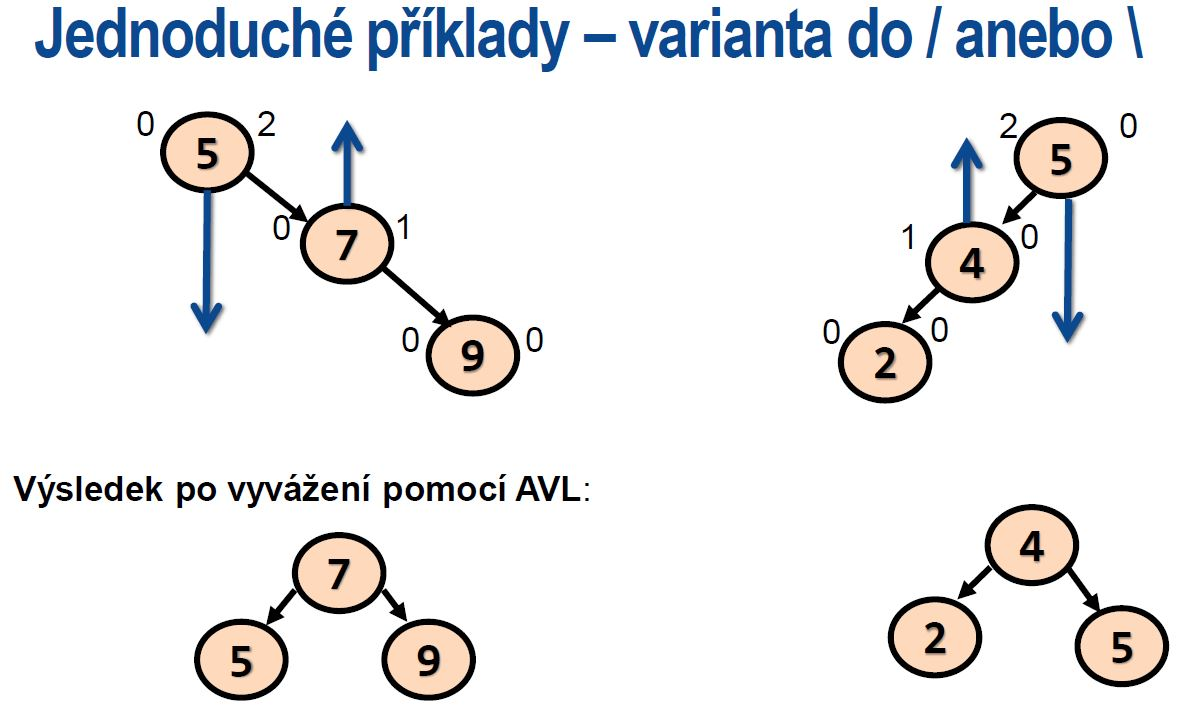
\includegraphics[width=\textwidth]{images/Rotation1Type.JPG}
		\caption{Rotace $\uparrow$ nebo $\downarrow$.}
	\end{minipage}
	\hspace*{1em}%
	\begin{minipage}[b]{0.47\textwidth}
		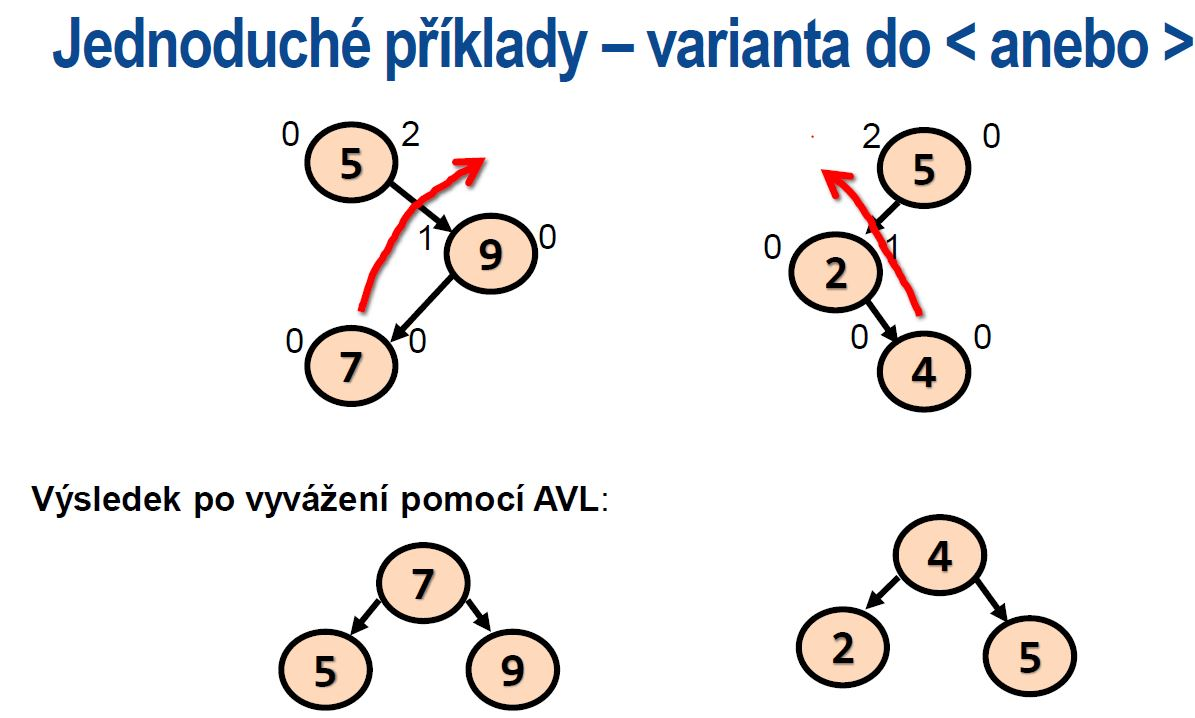
\includegraphics[width=\textwidth]{images/Rotation2Type.JPG}
		\caption{Rotace $\nearrow$ nebo $\nwarrow$.}
	\end{minipage}
\end{figure}

\subsection{Red-Black stromy}

Nejsou tak dobře vyvážené jako AVL, ale řeší problém mnohonásobné rotace. Efektivní vkládání, ale méně efektivní vyhledávání%
\footnote{Vizualizace \url{https://www.cs.usfca.edu/~galles/visualization/RedBlack.html}.}%
. Při vyvažování platí pravidla:
\begin{itemize}[noitemsep]
	\item Každý uzel je červený nebo černý.
	\item Kořen je vždy černý.
	\item Všechny listy jsou černé.
	\item Potomci červeného jsou vždy černí.
	\item Každá cesta z~libovolného uzlu do~jeho podřízených listů obsahuje stejný počet černých uzlů.
\end{itemize}

\section{Posouzení z~pohledu časové a~paměťové složitosti. ADT hashovací tabulky. Řešení kolizí hashovacích tabulek. Srovnání výkonnosti binárních vyhledávacích stromů a~hashovacích tabulek.}

\subsection{Hashovací tabulka}

Hashovací tabulka spojuje klíč s~odpovídající hodnotou. Klíč je vypočítán z~obsahu položky tak, aby byl klíč co nejjednoznačnější a~nedocházelo ke~kolizím; vše vychází z~pravděpodobnosti o~hashovacích funkcích. Využívají se~nejčastěji v~databázích nebo k~rychlému vyhledávaní v~polích. Paměťová složitost je O($n$).

\paragraph{Vkládání} Z~vkládaného prvku se udělá hash. Tento hash se~přiřadí do~pole, na~místo, které mu odpovídá. Jestliže je místo obsazeno přiřadíme mu další volné místo dle algoritmu.

\textbf{Vyhledávání} Využijeme klíče, který nám vrátí index položky. Jestliže na~odpovídajícím indexu se~nenachází daná položka, pomocí algoritmu vypočteme, kde je další místo, kde se~položka může nacházet.

\begin{table}[ht]
	\centering
	\caption{Časová složitost v~dobře a~špatně optimalizovaných tabulkách}
	\begin{tabular}{|c|c|c|}
	\hline
		Operace   & Průměrná & Nejhorší \\\hline
		Vkládání  & O(1)     & O($n$)   \\\hline
		Mazání    & O(1)     & O($n$)   \\\hline
		Vyhledání & O(1)     & O($n$)   \\\hline
	\end{tabular}
\end{table}

\subsubsection{Řešení kolizí}

\textbf{Řetězení tabulek}: Prvek je vložendo~lineárního seznamu.

\textbf{Otevřené adresování linear probing}: Prvek je vložen na další~vhodné místo. Zde si musíme hlídat, aby se~tabulka celá nenaplnila.

\textbf{Otevřené adresování double hashing}: Prvek je zhashován znovu.

\subsection{Hashovací tabulka vs binární strom}

\begin{table}[ht]
	\caption{Porovnání hashovací tabulky a~binárního stromu}
	\begin{tabularx}{\textwidth}{|l|X|X|}
	\hline
		  ADT & Výhody & Nevýhody \\\hline
		  Binární strom & Rychlé vkládání, mazaní a~hledání pokud je vyvažován & Algoritmus mazání je časově náročný. \\\hline
		  AVL a~Red-black stromy & Stejné jako binární stromy jen jsou vždy vyvážené takže optimální. & Jsou složité. \\\hline
		  Hashovací tabulka & Rychlé vkládání, při~existenci klíče rychlé vyhledávání. & Pomalý přístup pokud klíč není nalezen. Neefektivní využití paměti.\\\hline
	\end{tabularx}
\end{table}

Hashovací tabulka je rychlejší na~vyhledávání pokud je dobře napsána hashovací funkce, ve~špatném případě lze dojít ke~složitosti O($n$). Nelze vyhledávat pokud máme jen částečný klíč nebo potřebujeme v~nějakém intervalu. Další nevýhodou je složitost vytvoření hashovacích tabulek oproti stromu.

\clearpage
\section{Jednoduché a~pokročilejší řadící techniky a~jejich srovnání. Stabilita řadícího algoritmu. Bubble sort. Insertion sort. Selection sort. Shell sort. Merge sort. Heap sort. Quick sort.}

\subsection{Typy řazení}

\textbf{Řazení výběrem}: najde se~vždy nejmenší se~zbývajících prvků a~uloží se~na~konec už seřazených.

\textbf{Řazení vkládáním}: z~neseřazené množiny se~postupně bere prvek po~prvku a~vkládá se~na~správné místo přičemž začáteční množina už seřazených je prázdná.

\textbf{Řazení záměnou}: v~množině najdeme vždy dvojici, která je ve~špatném pořadí a~přehodíme ji.

\textbf{Řazení slučováním}: vstupní množinu rozdělíme na~části, které se~seřadí. Tyto seřazené části se~poté sloučí způsobem který vede k~seřazení.

\subsection{Porovnání algoritmů}

Třídění pomocí algoritmů Bubble Sort, Insert Sort a~Select Sort má složitost O($n^2$). Algoritmus Quick Sort má složitost $\Theta$($n\log{n}$), kdy v~nejhorším případě může nabývat až O($n^2$). Algoritmus Merge Sort má složitost O($n\log{n}$).

\subsection{Stabilita řízení}

Dělíme na~stabilní a~nestabilní. Vstupní data můžou obsahovat několik prvků se~stejnou hodnotou. Podle vzájemné polohy těchto prvků před a~po seřazení se~rozlišují tyto druhy. Stabilní algoritmus zachovává vzájemné pořadí položek se~stejnou hodnotou a~u nestabilního jejich zachování není zaručeno. Stabilní je vhodné využívat pokud řadíme podle dvou parametrů například jméno příjmení. Př. jestli řadíme osoby podle křestního jména a~poté podle příjmení tak Stabilní algoritmus by měl odpovídat očekávání. (První Karel Novák a~následoval by Václav Novák). Pokud bychom na~toto použili nestabilní algoritmus tak by druhé řazení mohlo zpřeházet výsledky prvního. (První by mohl být Václav a~až za~ním Karel.)

\subsection{Bubble sort}

Je jednoduchý stabilní řadící algoritmus se~složitostí O($n^2$).

Porovnávají se~dva sousední prvky, pokud je nižší číslo nalevo od~vyššího tak se~prohodí. A tak probublávají postupně dokud se~neseřadí. Pokud jsou čísla v~průběhu už správně seřazena tak je neprohodí ale postupuje dále.%
\footnote{Animace Bubble sort: \url{https://www.algoritmy.net/article/3/Bubble-sort}.}

\subsection{Insertion sort}

Je jednoduchý stabilní řadící algoritmus se~složitostí O($n^2$).

Máme jeden prvek a~ten vložíme do~už seřazené množiny, která je prázdná. Vezmeme následující prvek a~ten umístíme na~správné místo v~již seřazení množině. A takto pokračujeme dokud nedorazíme nakonec.%
\footnote{Animace Insertion sort: \url{https://www.algoritmy.net/article/8/Insertion-sort}.}

\subsection{Selection sort}

Je jednoduchý nestabilní řadící algoritmus se~složitostí O($n^2$).

Funguje na~principu výběru největšího prvku, který pak dá na~začátek. Pak vezme druhý největší a~ten dá nakonec seřazené části.%
\footnote{Animace Selection sort: \url{https://www.algoritmy.net/article/4/Selection-sort}.}

\subsection{Shell sort}

Je nestabilní kvadratický řadící algoritmus se~složitostí O($n^2$).

Funguje na~principu insertion sort. Rozdíl je v~tom že z~počátku neřadí prvky které jsou vedle sebe ale prvky které mají určitou mezeru mezi sebou. Tato mezera se~poté každou iteraci snižuje. Jak dojde na~mezeru 1 tak probíhá už pouze insertion sort.%
\footnote{Animace Shell sort: \url{https://www.algoritmy.net/article/154/Shell-sort}.}

\subsection{Merge sort}

Je stabilní složitý řadící algoritmus se~složitostí O($n\log{n}$).

Dělíme pole neustále na~poloviny dokud nemáme pole o~jednom prvku. Jakmile mám rozděleno na~jednotlivé prvky tak porovnám prvky vzájemně dva vedlejší prvky. Takže vzniknou pole o~dvou prvcích, které jsou už seřazené. Takto postupuji až k~začátku dělení. Jakmile má pole více elementů tak porovnám první prvek prvního pole s~prvním prvkem druhého pole a~seřadím je pokud je větší porovnám s~druhým prvkem prvního pole. Pokud je zase vetší tak je seřazeno. Pokud je menší tak ho přiřadím před druhý prvek prvního pole a~pokračuji s~druhým prvkem druhého pole. Ten už porovnávám pouze s~prvkem který byl vyšší než první prvek druhého pole. Tento proces opakuji dokud nedojdu k~seřazenému poli.%
\footnote{Video Merge sort: \url{https://www.youtube.com/watch?v=qdv3i6X0PiQ}.}

\subsection{Heap sort}

Je nestabilní složitý řadící algoritmus se~složitostí O($n\log{n}$). Je jeden z~nejefektivnějších řadících algoritmů.

Funguje na~principu prioritní fronty (stromová struktura). Prvně vytvoříme úplný binární strom (řazení vždy zleva doprava). Přetvoříme tento strom na~binární haldu/heap. nový heap vytvoříme tak že probubláváme prvky stromu od~nejnižších podstromů dle toho, jestli použijeme min/max heap při~min haldě bude kořenem vždy nejmenší číslo a~při max to bude naopak. Z~vytvořeného binárního stromu vezmeme kořen a~dáme ho do~množiny seřazených prvků a~v stromu přepíšeme kořen na~poslední element stromu. Tento strom zase řadíme dokud klidně opakovaně dokud nemáme na~každém kořenu min/max hodnotu. Tak pokračujeme dokud nezůstane žádný prvek.%
\footnote{Video Heap sort: \url{https://www.youtube.com/watch?v=LbB357_RwlY}.}

\subsection{Quick sort}

Je nestabilní složitý řadící algoritmus se~složitostí O($n^2$), resp. $\Theta$($n\log{n}$).

Prvně vybereme pivot (se špatně vybraným pivotem se~může zhoršit složitost). Dále všechny menší prvky než pivot přesuneme na~jednu stranu a~všechny vetší na~druhou. Dále vybereme nový pivot z~prvků na~levé straně a~provedeme stejný postup co ze~základním polem. To stejné uděláme s~pravou stranou. Pivot vždy zůstává na~místě a~nic se~s~nedělá, jelikož je považován za~setříděný. Tak postupuje dokud nám na~každé straně nezůstane jen jeden prvek.%
\footnote{Video Quick sort: \url{https://www.youtube.com/watch?v=ZHVk2blR45Q}.}

\clearpage
\section{Grafy, formální definice. Vyhledávání v~grafech. Algoritmus BFS (prohledávání do~šířky). Reprezentace BFS v~paměti. Algoritmus DFS (prohledávání do~hloubky).}

\subsection{Graf a~teorie grafů}

Graf je definován jako uspořádaná dvojice množiny vrcholů $V$~a~množin hran $E$ ($G(V,E)$), kde vrcholy (\emph{vertices/nodes}) jsou uzly grafu a~hrany (\emph{edges}) jsou spoje mezi vrcholy. Graf může být jakýkoliv rovinný nebo prostorový útvar, který bude znázorňovat důležité vazby mezi důležitými prvky (vrcholy).

\textbf{Hrana} znázorňuje vztah mezi vrcholy. Rozlišujeme na~hrany orientované a~neorientované. U~orientovaných lze stanovit počáteční a~koncový vrchol a~u neorientovaného to nelze. Hrany lze ohodnotit, kdy hodnota může například představovat délku, zátěž atd.

\textbf{Vrchol} je prvek, který chceme spojit s~druhým vrcholem pomocí hrany tak, aby nám vznikl graf (ne vždy tyto prvky musí být spojené). Vrchol lze ohodnotit; stupeň grafu je označení pro~počet připojených hran. Stupeň grafu je nejvyšší hodnota ze~všech stupňů jeho vrcholů. Grafy lze \textbf{dělit dle hran} na:

\begin{itemize}[noitemsep]
	\item Neorientované grafy obsahují pouze neorientované hrany. Hrana je obousměrná.
	\item Orientované grafy obsahují pouze orientované hrany. Hrana je pouze jednosměrná.
	\item Smíšené grafy obsahují oba typy hran.
\end{itemize}

\subsection{Vyhledávaní v~grafu}

\textbf{Druhy prohledávaní:}
\begin{itemize}[noitemsep]
	\item Slepé prohledávání: prohledávají náhodně bez~přemýšlení.
	\item Informované metody: snaží se~odhadnout, kudy pokračovat ve~vyhledávání aby byly co nejdříve v~cíli.
\end{itemize}

\paragraph{Nalezení kostry grafu spanning tree} Kostra grafu je nějaký strom, který neobsahuje cykly. Kostra se~vytváří tak, aby propojila všechny body a~celková váha byla co minimální. Při~hledání kostry s~co nejmenší váhou tento postup nazýváme minimal spanning tree. Nejznámějším algoritmem je Kruskalův algoritmus a~distribuovaný algoritmus.

\paragraph{Kruskalův algoritmus} Funguje na~principu shlukování dvou množin hran. Ze všech hran se~vybere hrana s~nejnižší hodnotou a~množiny vrcholů jenž hrana propojuje se~seskupí do~jedné množiny. Tak se~postupuje tak dlouho dokud všechny vrcholy nejsou v~jedné množině. Pokud cesta propojuje vrcholy ze~stejné množiny vrcholů tak se~nepoužije a~pokračuje se~z~následující hranou. Využívá se~pokud známe celou topologii grafu.%
\footnote{Animace Kruskal: \url{https://www.cs.usfca.edu/~galles/visualization/Kruskal.html}.}

\paragraph{Distribuovaný algoritmus} Zde se~pracuje na~principu, že se~kostra tvoří na~každé množině zároveň. Z~každého vrcholu se~vyrazí směrem po~nejmenší hodnotě hrany. Pokud se~vrcholy na~cestě potkají tak vytvoří množinu pokud se~nepotkají nic se~neděje. Dále se~pak vysílají znovu po~nejmenší hodnotě hrany. Toto se~děje dokud se~celá kostra nenajde. Tento algoritmus se~nejčastěji využívá v~telekomunikačních sítích, kde neznáme celou topologii grafu.

\begin{figure}[ht]
	\centering
	\includegraphics[scale=0.5]{images/distributed1.PNG}
	\includegraphics[scale=0.5]{images/distributed2.PNG}
	\caption{Distribuovaný algoritmus}
	\label{distributed}
\end{figure}

\subsection{Slepé prohledávání}

\textbf{BFS} využívá frontu do~které nejprve vloží vstupní vrchol. Z~tohoto vrcholu se~vezmou všichni sousedé a~vloží se~do~fronty, z~které se~bere postupně a~jejich sousedé se~přidávají do~fronty. Při~tomto se~každá už navštívený vrchol ukládá do~nějakého pole/seznamu navštívených abychom ho nenavštěvovali znovu.%
\footnote{Video BFS: \url{https://www.youtube.com/watch?v=oDqjPvD54Ss}}

\textbf{DFS}\,--\,pracuje na~principu, že prozkoumává prvně vrchol na~jednu stranu a~v ní pokračuje dokud nedojde na~konec nebo nedorazí do~už navštíveného vrcholu. Využívá zásobník.%
\footnote{Video DFS: \url{https://www.youtube.com/watch?v=pcKY4hjDrxk?t=279}.}

\vspace*{1em}

DFS je méně paměťově náročné, BFS je optimální.

\clearpage
\section{Omezené prohledávání do~hloubky (DLS). Iterativní prohledávání do~šířky (IDLS), Dijkstrův algoritmus (Uniform Cost Search), A*}

\subsection{Pokračování slepého prohledávání}

\textbf{DLS} vychází z~DFS, ale je omezen na~maximální hloubku.

\textbf{IDLS} je iterativní prohledávaní do~hloubky. Vychází z~DFS ale v~každé iteraci se~prohledává jen o~hloubku níž.%
\footnote{Video IDLS: \url{https://www.youtube.com/watch?v=Y85ECk_H3h4}.}

\textbf{Dijkstrův algoritmus} využívá prioritní frontu a~seznam navštívených vrcholů. Z~prvního vrcholu se~přidají všechny soudní vrcholy z~jejich hodnotou hrany do~prioritní fonty. Z~prioritní fronty se~vždy vezme nejmenší prvek. Z~nejnižšího vrcholu se~prozkoumají znovu sousedé ale tentokrát se~nepoužije pouze vzdálenost mezi nimi ale přičte se~už i~vzdálenost k~aktuálnímu vrcholu. Tak se~bere dokud se~nedorazí k~cílovému vrcholu.%
\footnote{Video Dijkstrův algoritmus: \url{https://www.youtube.com/watch?v=GazC3A4OQTE}.}

\subsection{A*}

\textbf{Informovaná metoda} A* využívá prioritní frontu a~seznam navštívených vrcholů. Každému z~vrcholů přidělíme vzdálenost od~cíle. Postupuje se~stejně jako u~Dijktrova algoritmu, akorát se sčítá vzdálenost s~hodnotu hrany. Dle této sečtené hodnoty je vybrán další navštívený prvek z~prioritní fronty.%
\footnote{Video A*: \url{https://www.youtube.com/watch?v=ySN5Wnu88nE}.}

\clearpage
\section{Evoluční algoritmy. Genetické algoritmy, genetické programování. Pojmy populace, mutace, křížení, chromozom. Princip evolučních algoritmů.}

Optimalizace a~jejími úlohami se~setkáváme při~řešení praktických úloh, při~kterých hledáme to nejlepší možné řešení. O nejlepším řešení se~rozhodujeme dle parametrů.

\subsection{Evoluční algoritmy}

Je jeden ze~způsobů optimalizace. Byly vytvořeny aby sjednotily optimalizační metody co využívají \enquote{evoluční} principy. Evoluční algoritmy zastřešují řadu přístupů využívajících modely biologické evoluce. Tyto modely jsou: přirozený výběr (výběr silnějšího jedince, podle fitness funkce), náhodný genetický drift (mutace, decimuje jedince s~vysokou fitness) a~reprodukční proces (křížení jedinců). Spadají zde přístupy jako genetické algoritmy, genetické programovaní, evoluční strategie, evoluční programovaní.

Obecný evoluční algoritmus začíná s~základní populací. Z~této populace se vytvoří výběr jedinců, které se zříží. Tito jedinci následně zmutují a~vytvoří novou populaci. Tyto kroky se~opakují v~$N$ iteracích. Ukončení je stanoveno předem: počtem iterací, dosažení požadovaného jedince, minimální změnou fitness populace po~několik iterací.

\subsection{Genetické algoritmy}

Genetické algoritmy jsou založeny na~Darwinově myšlence \enquote{přežije nejsilnější}. Využívá metody křížení, mutace a~selekce. Kódování řetězci má také svou analogii v~gentice, kde řetězce odpovídají chromozomům, jednotlivé pozice v~řetězci jednotlivým genům a~konkrétní hodnoty na~těchto pozicích pak alelám.

Genetické algoritmy začínají s~populací přípustných řešení, které jsou převedeny na~řetězce/pole. Poté jsou vybráni jedinci, kteří se budou podílet na~nové generaci: každý je ohodnocen fitness funkcí a~na~výsledku jsou vybráni nejvhodnější kandidáti (ale metod výběru je více). Tito jedinci se mezi sebou kříží a~na~konci cyklu mutují.

Výhody GA jsou že nevyžadují žádné speciální znalosti o~cílové funkci, jsou odolné proti klouzání do~lokálního optima. Mají problém s~nalezením přesného optima a~vyžadují velké množství vyhodnocování cílové funkce.

\subsection{Genetické programování}

Hledá samotnou funkci a~ne její parametry. Oproti GA se~liší v~reprezentaci jedinců. V~GP jsou jedinci vytvořeni stromem s~proměnlivou délkou chromozomu. Zjednodušeně je to převedení GA do~programovacích jazyků.

\subsection{Základní pojmy}

\textbf{Populace} je množina jedinců o~určité velikosti, ze~které jsou vybírání pro~operace (křížení, mutace atd.) při~evoluci. Konkrétní populace se~nazývá genotyp.

\textbf{Jedinec} člen populace, který je definován jedním chromozomem.

\textbf{Chromozom} je řetězec tvořený geny. Má za~úkol odlišovat se od~zbytku populace (DNA). Lze ho kódovat binárně, reálnými čísly, znaky, objekty, \dots

\textbf{Gen} na $i$-té pozici reprezentuje stejnou charakteristiku v~každém jedinci.

\textbf{Alela} je hodnota kterou může nabývat gen (např $\{0, 1\}$).

\textbf{Fitness funkce} kvantitativně vyjadřuje kvalitu každého řešení, např. dosažení požadované přesnosti algoritmu, množství času potřebné pro~výpočet algoritmu, množství chyb mezi skutečným a~požadovaným výstupem. Je více druhů metod vytvoření fitness funkce: hrubá, standardizovaná, přizpůsobená, normalizovaná.

\textbf{Selekce ruletový výběr, varianta 1}: pravděpodobnost výběru závisí na~kvalitě jedince (kolik místa na~ruletě zabírá). Pokud jedinec ostatní převyšuje výraznou měrou, nová populace bude tvořeny téměř výhradně geny. K~tomu se~využívají techniky potlačení/podpory.

\textbf{Selekce ruletový výběr, varianta 2}: jedinci jsou seřazeni vzestupně podle hodnoty fitness a~velikost místa je určena rovnicí. Tímto se~potlačují nadprůměrní jedinci, kteří by negativně ovlivňovali další generace.

\textbf{Selekce turnajový výběr}: náhodně se~vybere $n$ jedinců a~postupným porovnáváním je vybrán nejlepší.

\subsection{Metody křížení}

\begin{figure}[ht]
	\centering
	\includegraphics[scale=0.7]{images/elita.PNG}
	\caption{\textbf{Elitářství} zaručuje monotonní hodnotu fitness nejlepšího jedince a~předchází ztrátě nejlepšího řešení.}

	\includegraphics[scale=0.55]{images/1bod.PNG}
	\includegraphics[scale=0.55]{images/2bod.PNG}
	\caption{\textbf{n-bodové křížení} dělí genotyp v~$n$ bodech.}

	\includegraphics[scale=0.7]{images/uniform.PNG}
	\caption{\textbf{Uniformní křížení} rozvrací kód chromozomu a~je dobré pro~vnáščení diverzity.}

	\includegraphics[scale=0.7]{images/mutace.PNG}
	\caption{\textbf{Mutace} se aplikuje s~malou pravděpodobností a~je důležitá především pro~malé počty jedinců.}
\end{figure}

\section{Paralelní výpočty a~architektury, procesy, vlákna a~jejich synchronizace, Deadlock.}

Sériové výpočty běží na~jediném CPU s~použitím jednoho vlánka, kde je problém rozdělen na~posloupnost instrukcí. Každá instrukce se~vykonává postupně, kdy v~daném času může být spuštěna pouze jedna instrukce.

\textbf{Paralelní výpočty} na~rozdíl od~sériových běží na~několika CPU. Zde jsou problémy rozděleny na~části a~až tyto části problému jsou rozděleny na~posloupnost instrukcí. Instrukce každého problému jsou poté vykonávány souběžně na~několika CPU.

\begin{figure}[ht]
	\centering
	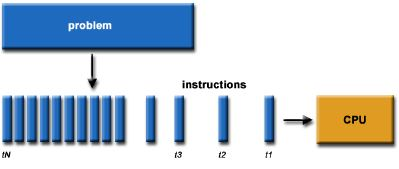
\includegraphics[scale=0.7]{images/serialComputing.JPG}
	\hspace*{1em}
	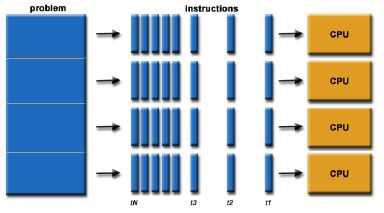
\includegraphics[scale=0.7]{images/parallelComputing.JPG}
	
	\caption{Sériové a~paralelní výpočty}
\end{figure}

Veškeré paralelní výpočty lze provádět sekvenčně, ale ne všechny sekvenční algoritmy lze paralelizovat. Příklady výpočetních zdrojů:
\begin{itemize}[noitemsep]
	\item Počítač s~několika procesory
	\begin{itemize}[noitemsep]
		\item Multiprocesor se~sdílenou pamětí (propojení více procesorů dohromady)
		\item Multiprocesor obsahující několik procesorů (jader) na~jednom čipu (obyčejné CPU).
	\end{itemize}
	\item Libovolný počet počítačů propojený počítačovou sítí (Cluster computer)
	\item Spojení výše uvedeného do~jednoho systému.
\end{itemize}

\subsection{Sériové a~paralelní modely (architektura)}

Modely dělíme hlavně dle Flynnovy klasifikace z~dvou hledisek: toku instrukcí a~toku dat.

\begin{table}[ht]
	\centering
	\caption{Modely dle Flynnovy klasifikace}

	\begin{tabular}{c|cc}
	{}            & Single Intruction & Multiple Instructions \\
	\hline
	Single Data   & sériový           & paralelní             \\
	Multiple Data & paralelní         & paralelní             \\
	\end{tabular}
\end{table}

\paragraph{SISD}

Nejjednodušší model, který si lze představit jako (jednojádrový) procesor. Vykonává pouze jednu instrukci nad~jedinými daty uloženými v~paměti. Instrukce jsou posílány do~řídící jednotky z~paměti, následně jsou dekódovány a~poslány procesní jednotky. Ta tyto data zpracuje a~pošle je zpátky.

Nejčastěji se~vyskytuje v~počítačích založených na~von Neumann architektuře.

\paragraph{SIMD}

Systémy, u~kterých existuje celá řada zpracovaných datových toků na~základě jediného seznamu instrukcí. V~každém okamžiku veškeré procesory vykonávají stejnou instrukci, kdy každá výpočetní jednotka může pracovat s~libovolnými daty. Tento model je vhodný pro~problémy, kde je charakteristická velká míra pravidelnosti (zpracovaní obrazu/videa, násobení matic). Existují dvě varianty v~podobě procesorového pole a~vektorové \enquote{potrubí/pipeliny}.

Příklad sčítání dvou polí vektorů. Pole jsou rozděleny na~bloky a~každý procesor pracuje s~daným blokem. Položky jsou poté vybírány na~základě ID procesu/vlákna.

\begin{figure}[ht]
	\centering
	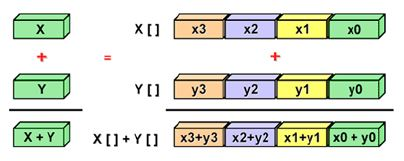
\includegraphics[scale=0.7]{images/SIMD.JPG}
\end{figure}

\paragraph{MISD}

Jeden datový proud je napojen na~několik procesorů. Každý procesor pracuje se~stejnými daty, ale může s~nimi vykonávat jiné operace. MISD jsou vhodné pro~vícenásobné frekvenční filtry pracující na~jednom signálovém proudu nebo kryptografické algoritmy pokoušející se~prolomit jednu zakódovanou zprávu.

Lze je použít například ve~vícenásobných vyhledávacích algoritmech, kde tyto algoritmy mohou pracovat se~stejnými daty. Také mohou tyto algoritmy používat různou strategii a~hledat různé vzory.

\paragraph{MIMD}

Tento model umožňuje zpracovávat různé posloupnosti instrukcí a~pracovat s~různými daty. Spouštění může být synchronizované, asynchronizované, deterministické nebo nedeterministické.

Jsou vhodné pro~intenzivní paralelní výpočty. Tento model se~využívá ve~většině superpočítačů a~výpočetních klusterech propojených přes síť.

\subsection{Architektura paralelní počítačové paměti}

\paragraph{Sdílená paměť}

Umožňuje všem procesorům přístup ke~všem pamětím jako globálnímu adresovému prostoru. Procesory mohou pracovat nezávisle a~sdílet stejné paměťové prostředky, změna paměti je viditelná všem procesorům.

\paragraph{Distribuovaná paměť}

Vyžadují komunikační síť pro~propojení meziprocesorové paměti. Každý procesor má vlastní lokální paměť (tj. neexistuje sdílená paměť jako v~předchozím případě). Procesory pracují nezávisle a~je na~programátorovi aby zajistil synchronizaci dat.

Výhodou je škálovatelnost s~počtem procesorů a~rychlý přístup k~paměti. Nevýhodou je zodpovědnost programátora za~spousty detailů při~synchronizaci procesů.

\paragraph{Hybridní distribuovaná sdílení paměť}

Využívá se~obvykle SMP (Symetrické MultiProcessory: HW architektura kde více procesorů sdílí jeden paměťový prostor). Procesory na~daném SMP mohou adresovat paměť tohoto procesoru jako globální. SMP znají pouze vlastní paměť a~ne jiného SMP. Pro přesun dat se~využívá sítová komunikace.

\subsection{Paralelní programovací modely}

\paragraph{Sdílená paměť}

Úkol sdílí společný adresní prostor, který čte a~zapisuje asynchronně. Výhodou je neexistence vlastnictví, takže není výslovně potřebné specifikovat komunikaci dat mezi úkoly. Řídit přístup ke~sdílené paměti lze pomocí zámků a~semaforů.

\paragraph{Vláknový model}

Jeden proces může mít více souběžných cest provádění. Vlákno lze popsat jako podprogram v~rámci hlavního programu, kde má každé vlákno lokální data a~kde mezi sebou vlákna komunikují pomocí globální paměti. Mezi vlákny musí být zajištěna synchronizace aby nedošlo k~přístupu ke~stejné globální adrese více jak jedním vláknem.

\subsection{Procesy a~vlákna}

\textbf{Vlákna} jsou méně náročná na~systémové prostředky, sdílí paměť, snadnější programování, ale mají omezenou škálovatelnost. \textbf{Procesy} jsou náročnější na~vytvoření, komunikace probíhá předáváním zpráv (nesdílí data), jsou náročnější na~programování, ale dobře se škálují.

\paragraph{Synchronizace vláken}

Bez zajištění synchronizace může dojít k~souběhu nebo uváznutí (deadlock). Cílem synchronizace je zabránit konfliktům mezi vlákny při~přístupu ke~sdíleným prostředkům.

\paragraph{Souběh}

K~souběhu dochází v~případě, kdy ke~stejným datům přistupuje více vláken a~jedno druhému přepíše data. Tím vzniká chyba za~běhu programu.

\paragraph{Deadlock}

Nastává v~případě, kdy na~sebe dvě vlákna nebo dva procesy čekají na~situaci, kdy se jim uvolní vzájemně uzamčené zdroje. Stává se při~nesprávném použití synchronizačních mechanismů. Je nedeterministický a~tedy obtížně testovatelný.
